\appendix
\chapter{Running the code}
\section{BON Extractor}
The textual \bon{} extractor is a part of EiffelStudio, more specifically, the Eiffel Verification Environment, or \textsc{eve} for short. Therefore, to run the extractor one needs to install\textsc{eve}. An instruction for this can be found at the \textsc{eve} website \url{http://eve.origo.ethz.ch/} or on the attached \textsc{cd} (\textit{EVE Setup.html}). It is important to note that the latest version of \textsc{eve} requires a new version of the Eiffel compiler (EiffelStudio 7.1). This can be found at \url{http://dev.eiffel.com/Downloads} in the beta area.

\paragraph{}
When in \textsc{eve} the textual \bon{} views should show up along side the others as seen in figure \ref{fig:EiffelStudio1}.

\begin{figure}[H]
\centering

\includegraphics[scale=0.8]{images/es1.png}
\caption{EiffelStudio picture 1}
\label{fig:EiffelStudio1}
\end{figure}

Should they not, right click a tool bar to and select "Customize Address Toolbar" as seen in figure \ref{fig:EiffelStudio2} .

\begin{figure}[H]
\centering
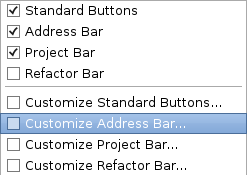
\includegraphics[scale=0.8]{images/es2.png}
\caption{EiffelStudio picture 2}
\label{fig:EiffelStudio2}
\end{figure}

A window similar to the one in figure \ref{fig:EiffelStudio3} should pop up. In this window select the \bon{} views and add them to the toolbar. Optionally, move them to the other views.

\begin{figure}[H]
\centering
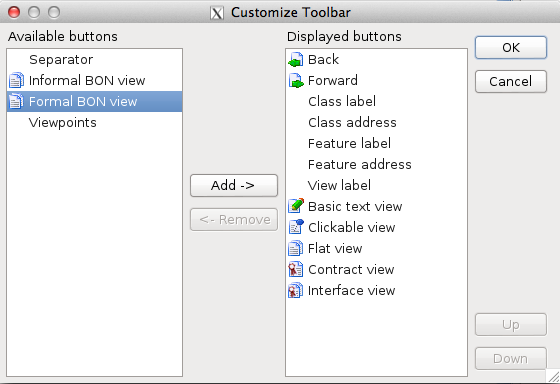
\includegraphics[scale=0.8]{images/es3.png}
\caption{EiffelStudio picture 3}
\label{fig:EiffelStudio3}
\end{figure}

\section{Type checker}

\import{./}{specification-type-system}
\import{./}{standard-types}
\chapter{Components not extracted}
\label{components-not-extracted}
Some elements are not extracted by the textual \bon{} extractor. Below is a list of omitted elements. Any subelement of an excluded are also excluded. The elements are shown as they appear in \cite[pp. 352--359]{walden1995}.\newline\newline

\noindent\textbf{Event\_chart}\newline
In textual \bon{} an event charts purpose is to express important events. As extracting semantics from source code is out of this projects scope, it has been omitted.\newline\newline

\noindent\textbf{Scenario\_chart}\newline
Similar to event charts, scenario charts purpose is to express semantics.\newline\newline
  
\noindent\textbf{Creation\_chart}\newline
Creation charts could have been included, but it would have been very involving as a lot of further analysis would have been required. This is a possibility for a future project.\newline\newline
  
\noindent\textbf{Static\_relations}\newline
Similar to creation charts, static relations could have been included, but as with creation charts, it's something for further development.\newline\newline

\noindent\textbf{Dynamic\_diagram}\newline
Since dynamic diagrams, as the name implies, describe a dynamic context, our static analysis would not be able to make sensible dynamic diagrams.\newline\newline

\noindent\textbf{Class\_dictionary}\newline
Class dictionaries could have been included to give further overview over a system, however it was deemed unnecessary due to its similarity to informal charts. Thus, there were more interesting parts of the project to dedicate time to.\newline\newline

\noindent\textbf{Part}
The reason for parts omission was discussed in section \ref{part}.

\import{./}{extraction-example}
